\documentclass{article}

% Includes preamble from standard file
% ==========================================================
%   GPR-20 MANUALS PREAMBLE
% ==========================================================

% ==========================================================
% Includes packages
\usepackage{float}
\usepackage{amssymb}
\usepackage{parskip}
\usepackage{caption}
\usepackage{booktabs}
\usepackage{tabularx}
\usepackage{titlesec}
\usepackage{hyperref}
\usepackage{enumitem}
\usepackage{setspace}
\usepackage{graphicx}
\usepackage{xltabular}
\usepackage{longtable}
\usepackage{csvsimple}
\usepackage{subcaption}
\usepackage{indentfirst}
\usepackage[utf8]{inputenc}
\usepackage[margin=1in]{geometry}
\usepackage[type={CC}, modifier={by-nc}, version={4.0}]{doclicense}
\usepackage{subfiles}
% ==========================================================

% ==========================================================
% PREAMBLE SETTINGS
% Sets double spacing
\doublespacing

% Sets paragraph indentation
\setlength{\parindent}{1em}

% Sets paragraph skip
\setlength{\parskip}{2em}

% Sets the list separation
\setlist{nosep}
% ==========================================================


% Adds bibliography
\usepackage[style=numeric]{biblatex}
\bibliography{biblio.bib}


% Defines command to insert name
\newcommand{\GPRManualName}{Field Setup Manual}

% ==========================================================
% DOCUMENT INFORMATION
\title{GPR-20: Field Setup Manual}
\author{Grupo de Desminado Humanitario}
\date{July 2021}
% ==========================================================

\begin{document}

\subfile{front}

\newpage
\section{Introduction}
This document presents the field setup and use protocol for the GPR-20 robot. The field setup protocol is designed to ensure that the robot will be properly configured on a remote location. The scope of this document includes preliminary checks, transportation, field assembly and disassembly, testing of the robot, parameters configuration, and survey supervision. Each step addressed in this document must be carefully executed in order to prevent permanent damage to the robot or erroneous data. Not following this document directions could result in the robot not performing as expected during data acquisition. 

Transport of the robot and recommendations of this process are also addressed in the document. Not following the transport recommendations could result in permanent damage of the robot. Damage during robot transport could also result in failing to acquire data in the field. This would happen if no replacement parts are available in the surveying location. However, no damage should occur if the indicated practices are followed. 

A manual on the robot assembly and disassembly on field is provided in this document. The manuals are stated in such a way that they can be filled as a checklist. Assembly of the robot starts with the major components manufactured, assembled and configured and stops with the robot ready to perform the field testing. Disassembly of the robot follows the opposite path. 

Testing is defined in order to check the robot performance before acquiring data. This procedure ensures that acquired data will be homogeneous among different measurements in different locations. Testing includes checking the robot pose, calibrating the VNA instrument and taking a test measurement under a predefined standard condition. 

Checking the robot pose ensures that the robot will be leveled among the earth surface to avoid excessive load on the robot motors. Calibrating the VNA instrument is required to execute the data acquisition under a standard setup of the instrument. Finally, the test measurement is used to check if acquired data is consistent with theoretical predictions.

After testing is performed, the robot must be configured for the data acquisition process. In this stage, the survey parameters are entered by the user interface. Once configured, the data acquisition process can start. Although the robot will automatically acquire the data without the user intervention, it is recommended that the user supervises the process. This manual presents considerations regarding the survey supervision.

The reader should read the whole manual before interacting with the robot and keep it handy during field setup. The manual includes a set of checklists that must be followed during any field assembly/dissemble setup to ensure that the robot will suffer no damage. Each assembly procedure must have its own filled checklist for robot-keeping purposes.

\newpage
\section{Robot Preliminary Checks}
This manual assumes that the robot is disassembled in its major components and it has been transported to measurement location. If robot is assembled and it is not in the measurement location, please follow the disassembly and storage procedures. By following this procedures you will make sure that the robot and its components will not be damaged. If robot is already assembled in the measurement location, please refer to testing procedure.

Since data is acquired from remote locations, the robot itself requires an environment that provides power and shelter. Power consists of a electricity supply that can be directly from the grid or by using a generator. If a generator is used, it must be kept within XX meters from the robot to avoid electromagnetic interference. Shelter must be provided to avoid damage from adverse weather. 

\subsection{Electronics Box Preliminary Checks}
\begin{figure}[H]
    \centering
    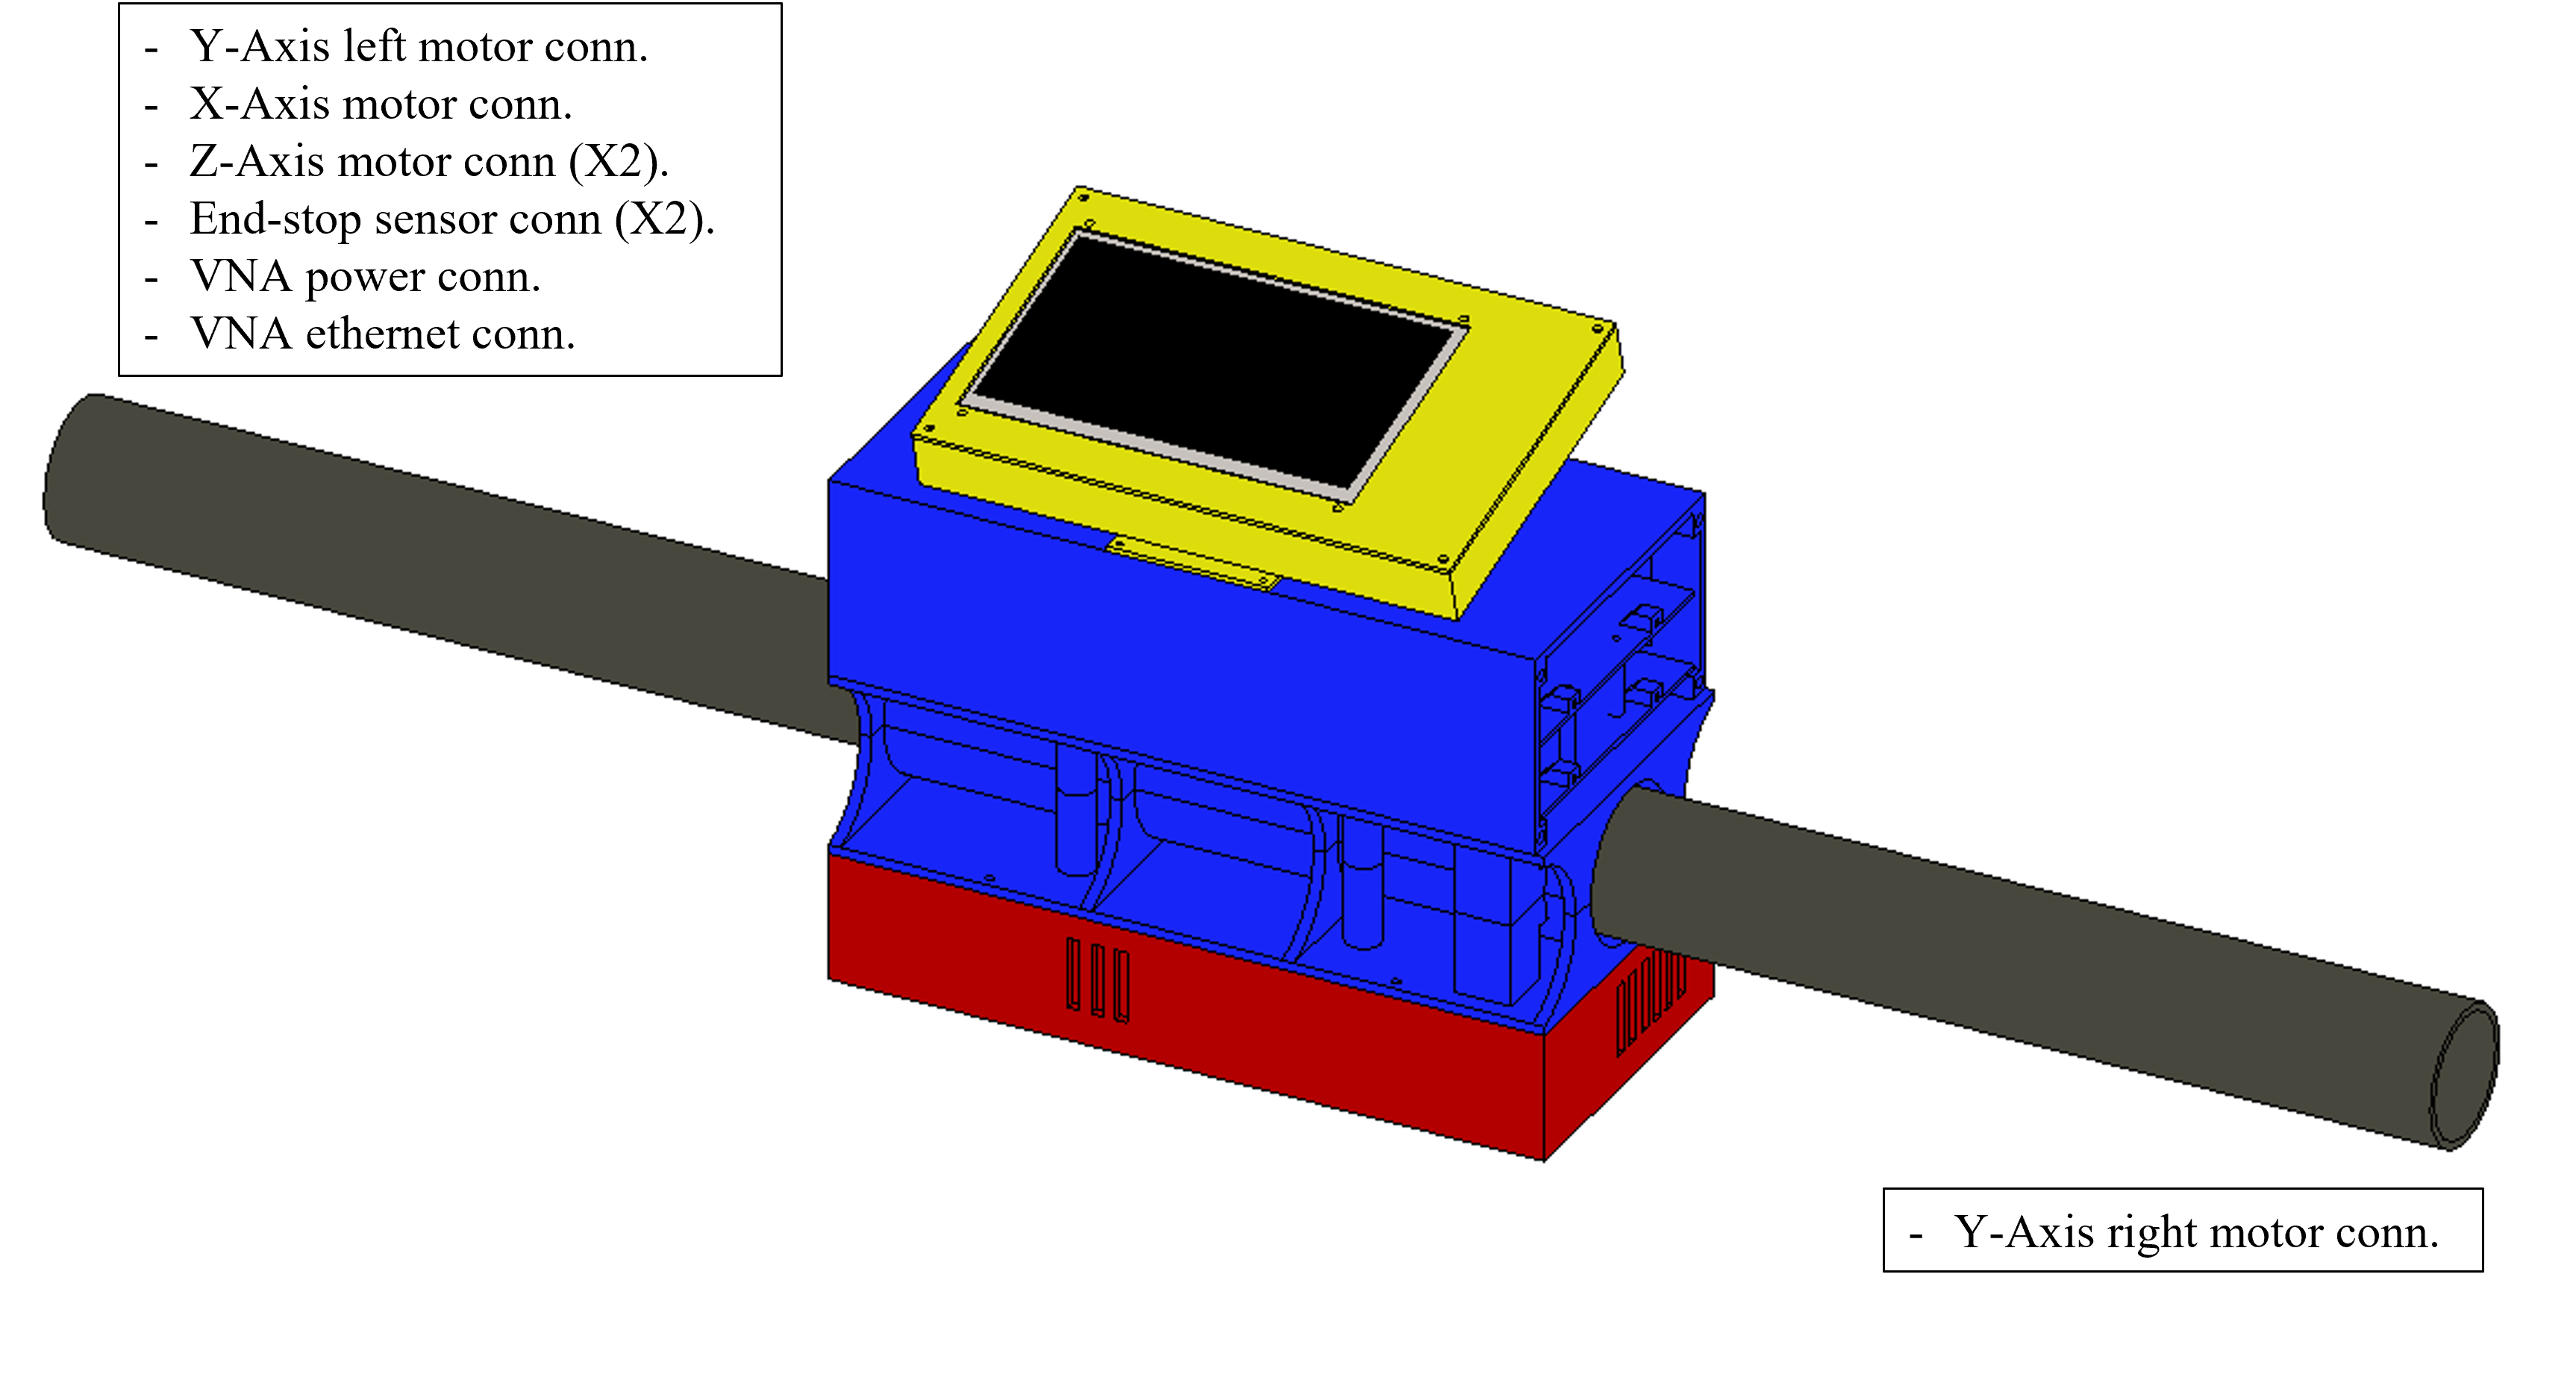
\includegraphics[width=0.8\textwidth]{images/requirements/text_eb.png}
    \caption{Electronics box with its connectors identified.}
    \label{fig:considerations_electronics_0}
\end{figure}
The electronics box consists of a case for the electronic systems of the robot mounted on a two-inch PVC pipe. The electronics box connects to the robot through a set of different connectors. There are nine (9) connectors located at the end of the PVC pipe. To identify the connectors place the PVC pipe with the electronics box with the touchscreen facing you as shown on figure \ref{fig:considerations_electronics_0}. On the right end of the pipe there is only one connector: the phases for the right Y-axis motor. The left side has eight (8) connectors: 
\begin{itemize}
    \item Phases for left Y-axis motor.
    \item Phases for X-axis motor.
    \item Phases for two Z-axis motors.
    \item Power and data lines for Y-axis endstop sensor.
    \item Power and data lines for X-axis endstop sensor.
    \item Power lines for VNA instrument.
    \item Ethernet lines for VNA instrument.
\end{itemize}

\subsection{Y-Axes Preliminary Checks}
\begin{figure}[H]
    \centering
    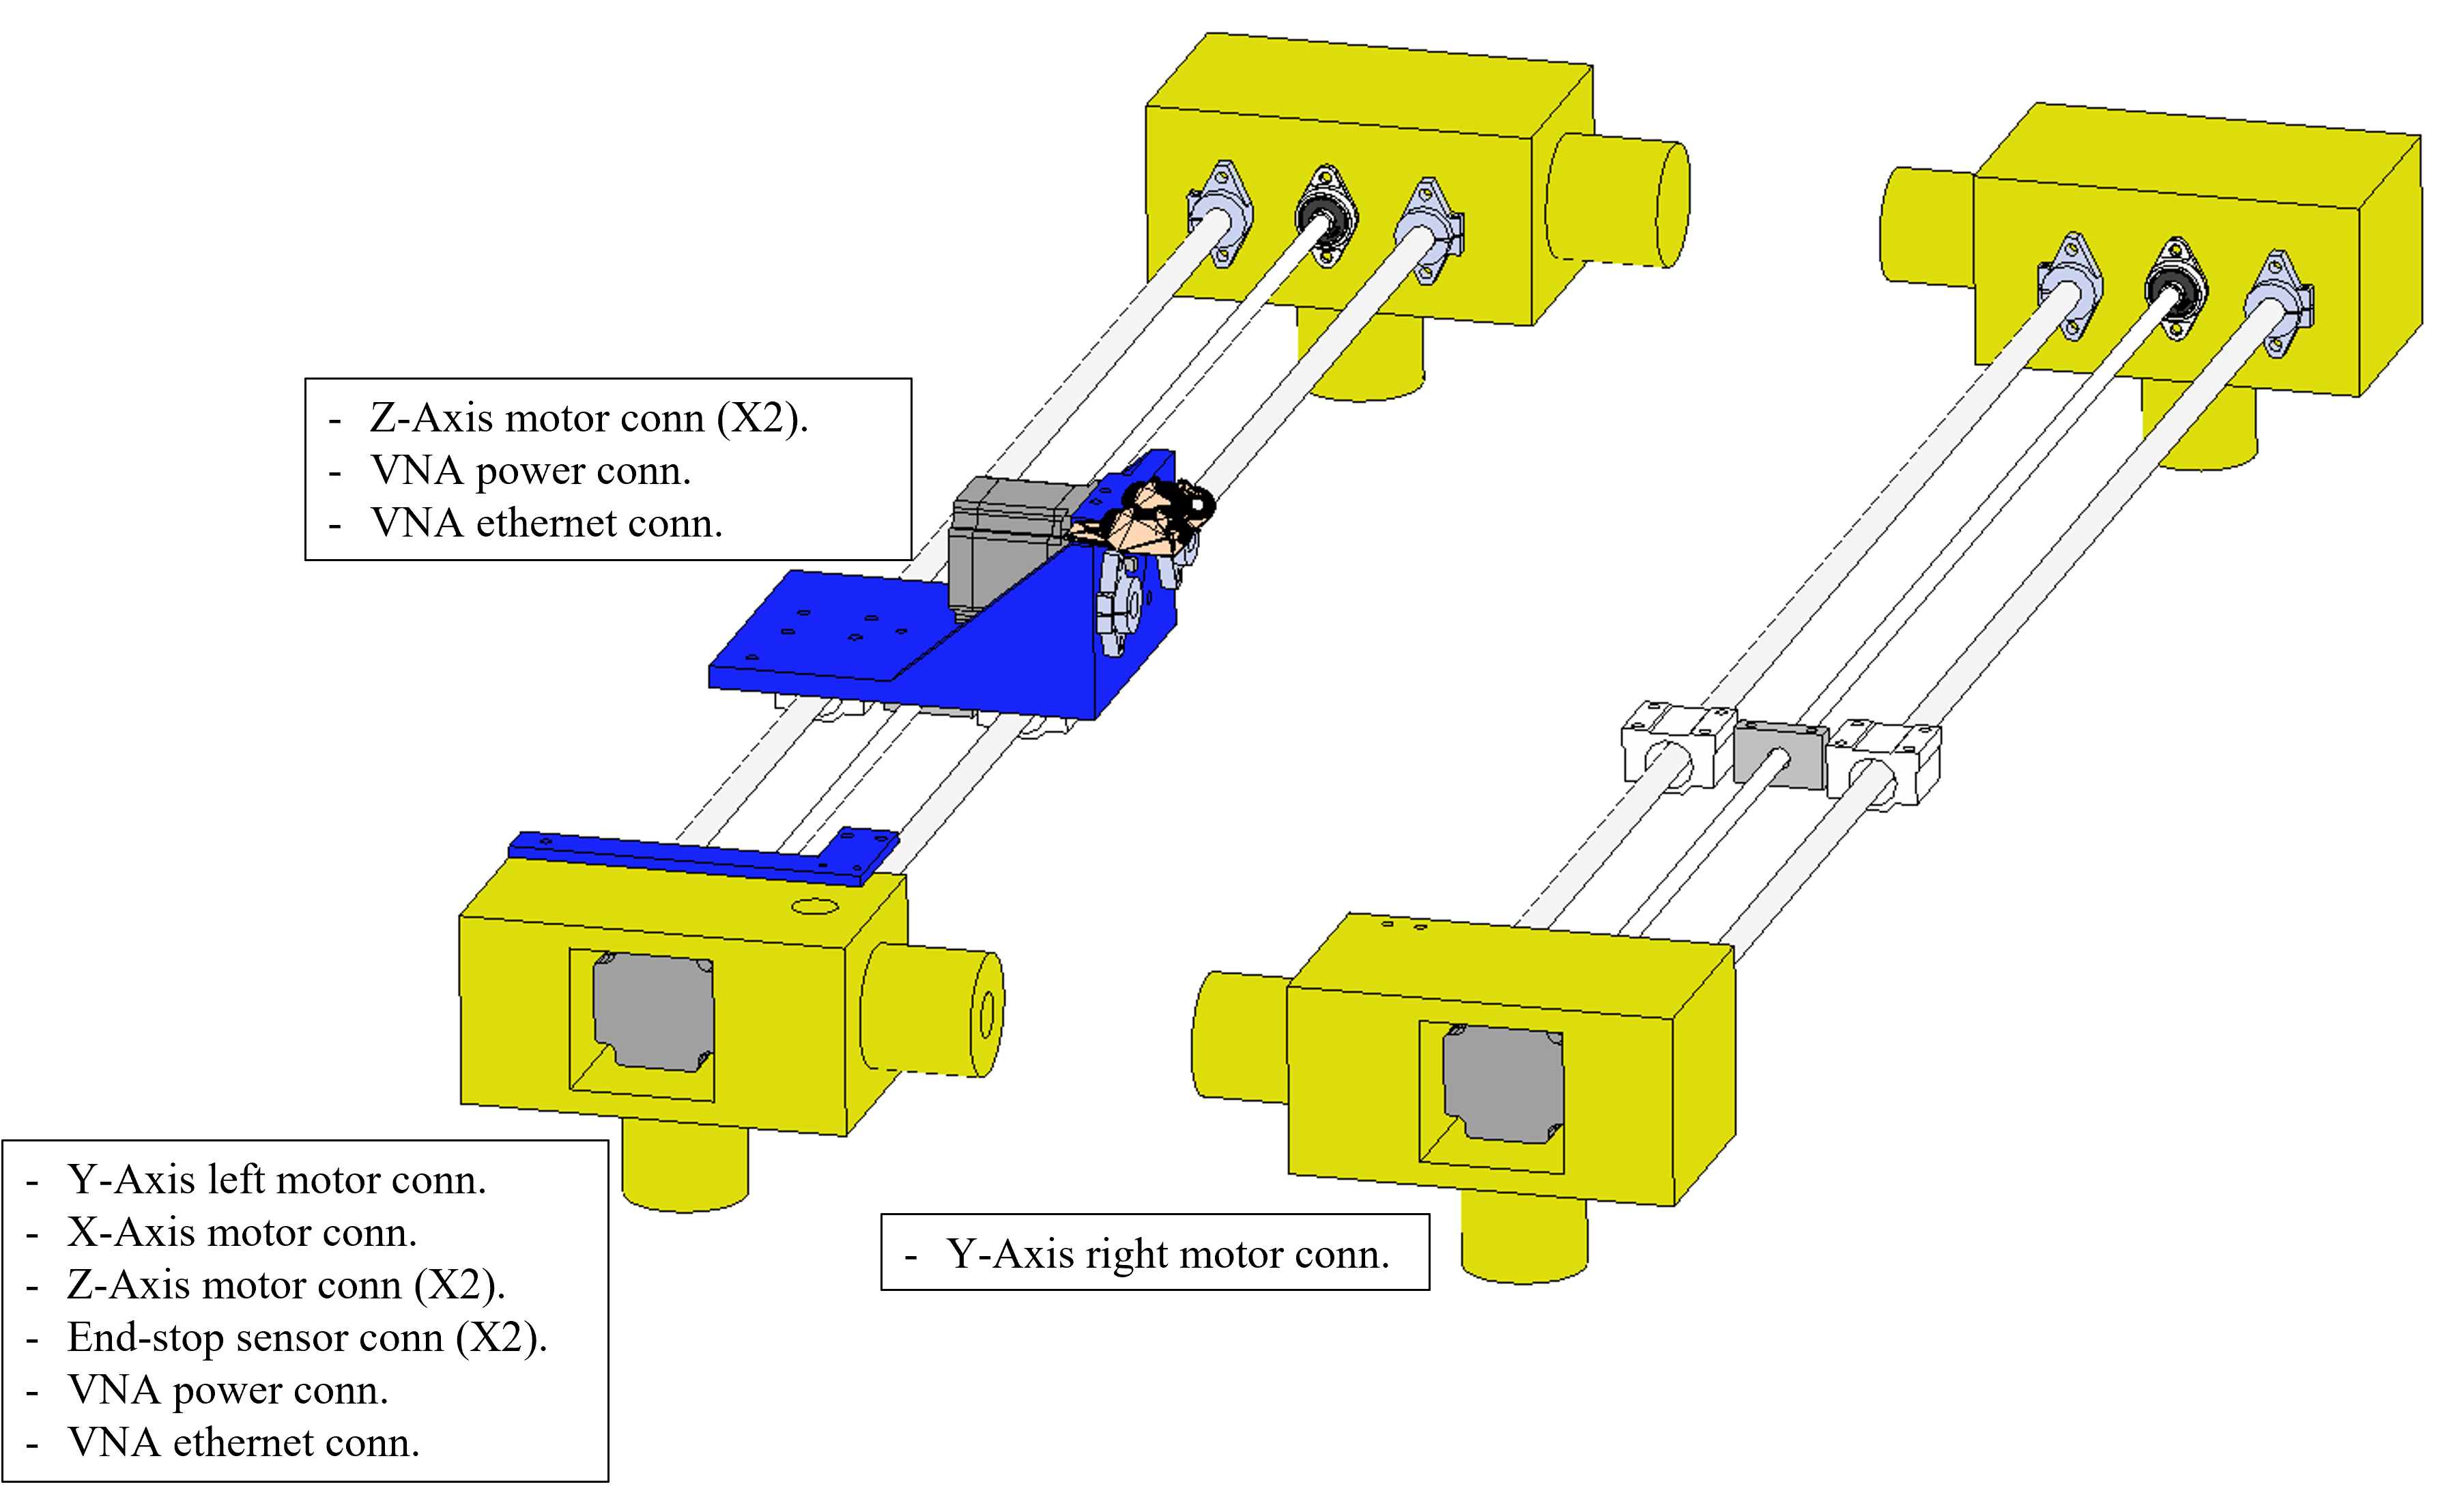
\includegraphics[width=0.8\textwidth]{images/requirements/text_yaxes.png}
    \caption{Y-Axis arms with their connectors identified. Note that the X-Axis support is not a part of this major component.}
    \label{fig:considerations_y_arms_0}
\end{figure}
The Y-Axis arms are two linear actuators that move the GPR over the defined Y axis of the robot. They consist of two 3D-printed end support elements connected by two one-meter rods and a linear screw. At one end of each arm there is a support element with a stepper motor. Each motor support element has a hollow PVC tube support in which a connector set is located. The right Y-Axis arm has only one connector: the phases for the right Y-axis motor. The left arm has an additional connectors set on the X-Axis motor mount. The connectors for the left Y-Axis arm support element are:
\begin{itemize}
    \item Phases for left Y-axis motor.
    \item Phases for X-axis motor.
    \item Phases for two Z-axis motors.
    \item Power and data lines for Y-axis endstop sensor.
    \item Power and data lines for X-axis endstop sensor.
    \item Power lines for VNA instrument.
    \item Ethernet lines for VNA instrument.
\end{itemize}
And the connectors on the X-Axis motor mount located on the left Y-Axis arm are:
\begin{itemize}
    \item Phases for two Z-axis motors.
    \item Power lines for VNA instrument.
    \item Ethernet lines for VNA instrument.
\end{itemize}

\subsection{X-Axis Preliminary Checks}
\begin{figure}[H]
    \centering
    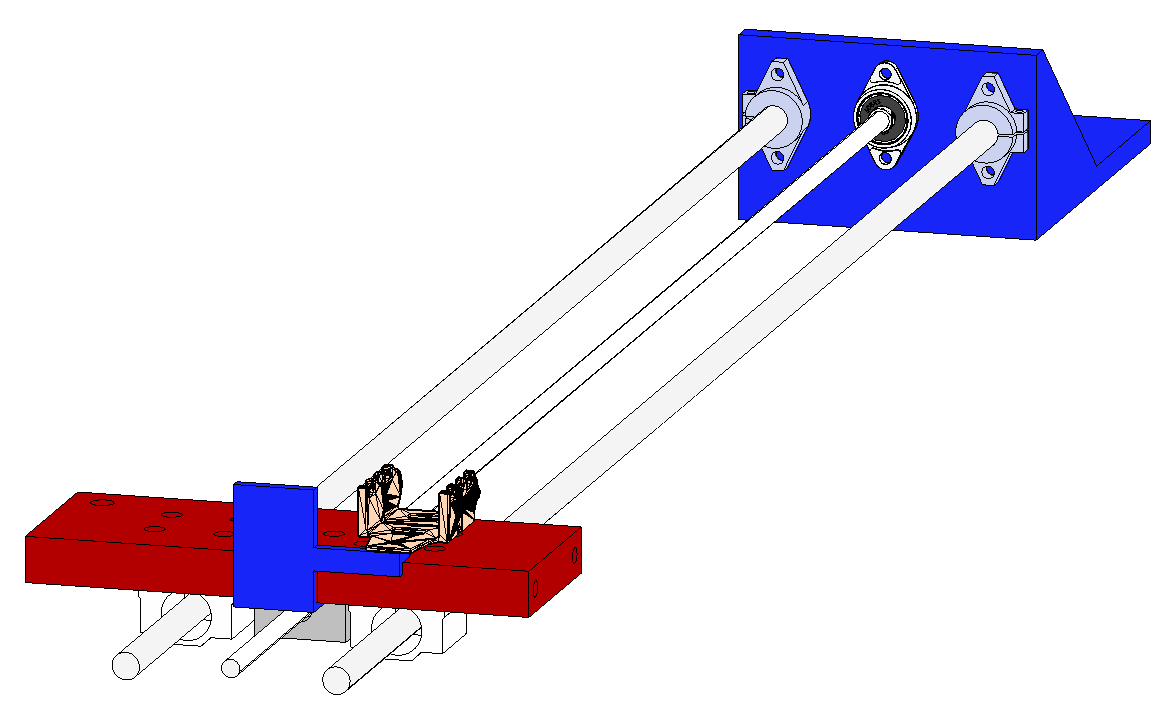
\includegraphics[width=0.8\textwidth]{images/requirements/x_axis.png}
    \caption{X-Axis arms with their connectors identified.}
    \label{fig:considerations_x_arm}
\end{figure}
The X-Axis arm is a linear actuator, similar to the Y-Axis arms.The X-Axis consists of a 3D-printed motor mount and a support element that are connected together by a pair of rods and a linear screw. The movable part of the X-Axis is denoted as an universal mount for the GPR support structure. The initial links of a drag chain are attached to the X-Axis arm. The remaining part of the drag chain and the cables are part of the GPR support structure. GPR-20 X-Axis arm is shown on figure \ref{fig:considerations_x_arm}. Note how the beginning of the drag chain is attached to the universal mount.

\subsection{VNA Holder Preliminary Checks}
\begin{figure}[H]
    \centering
    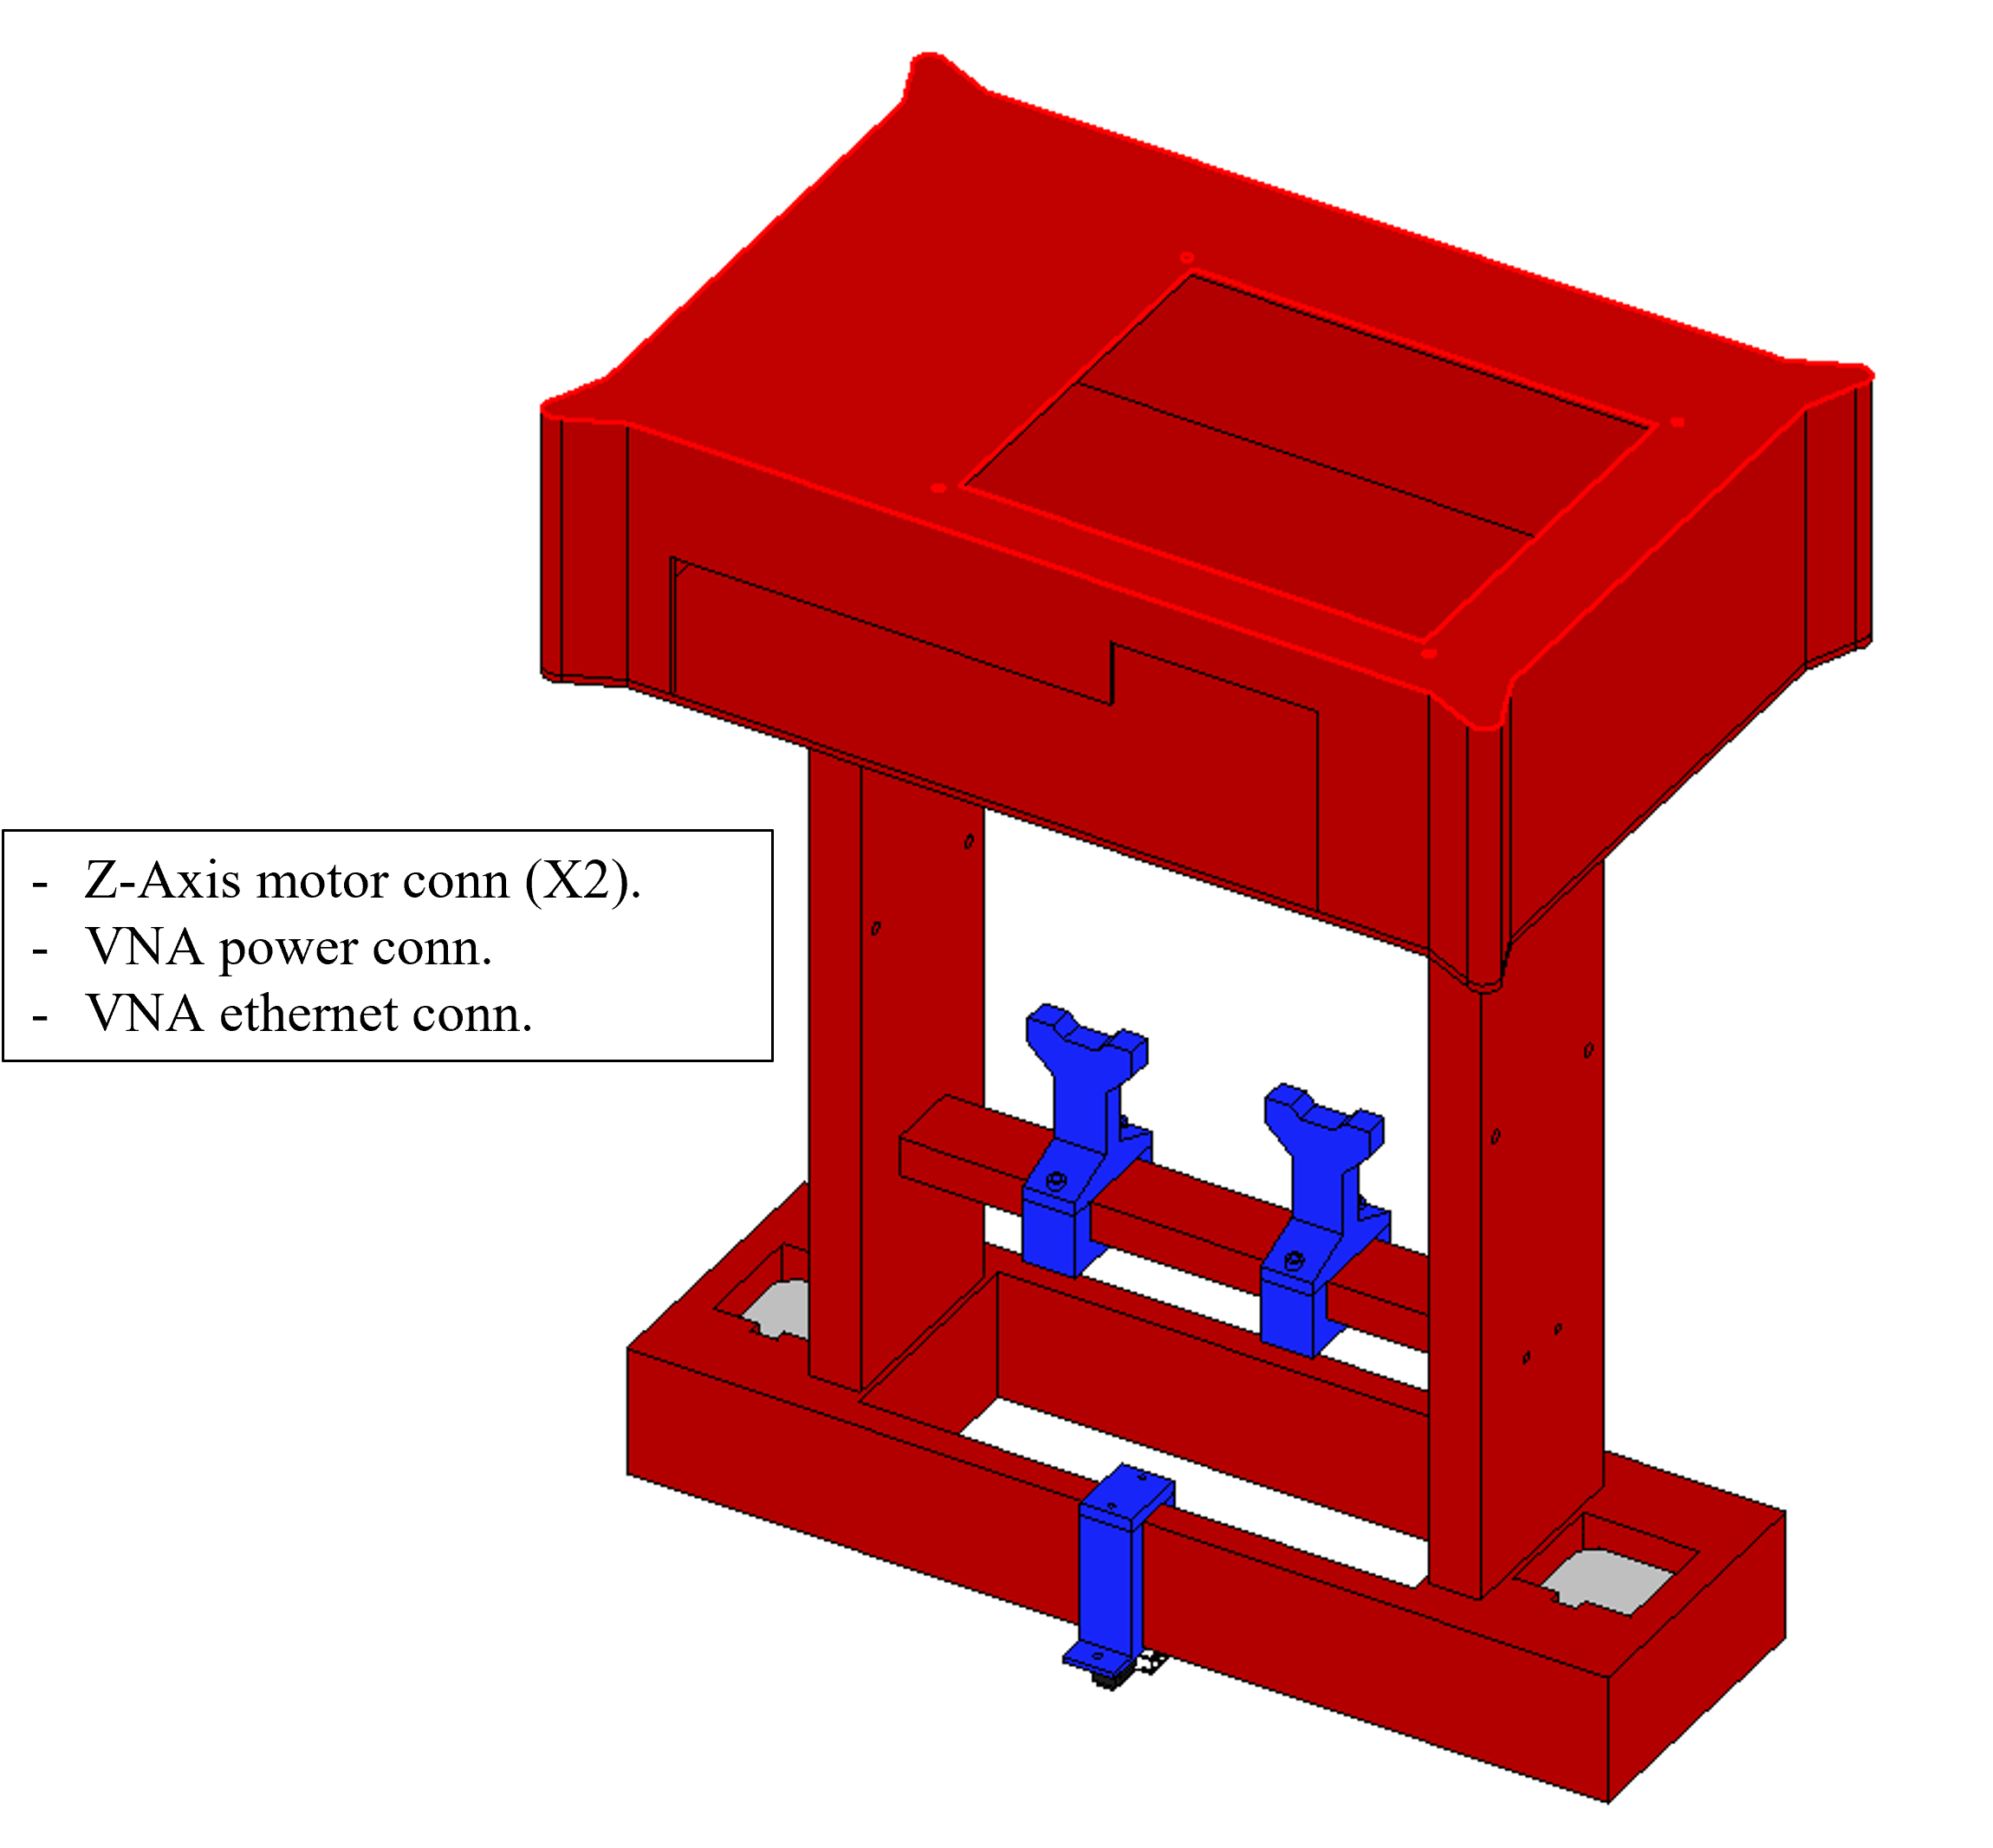
\includegraphics[width=0.8\textwidth]{images/requirements/text_gpr.png}
    \caption{GPR support structure.}
    \label{fig:considerations_gpr}
\end{figure}
The GPR structure are the mechanical elements that provide support for the vector network analyzer (VNA) and the antennae. Antennae on the GPR-20 can rotate 90 degrees to acquire data in different polarization thus require two stepper motors. The GPR support structure requires four connections:
\begin{itemize}
    \item Ethernet connection for VNA data.
    \item Power connection for VNA power.
    \item Phases for two Z-axis motors.
\end{itemize}
The cables and the connections are stored using the X-Axis drag chain. The X-Axis drag chain ends are attached to the left Y-Axis arm (X-Axis motor mount) and the X-Axis arm (Universal Mount). 

\subsection{Ground Support Preliminary Checks}
Figure \ref{fig:considerations_ground_supports} presents the ground support elements for the GPR-20 robot. The free end of the PVC tubes must be inserted in the Y-Axis support elements. Make sure to test if the PVC tube can be inserted in the support element.
\begin{figure}[H]
    \centering
    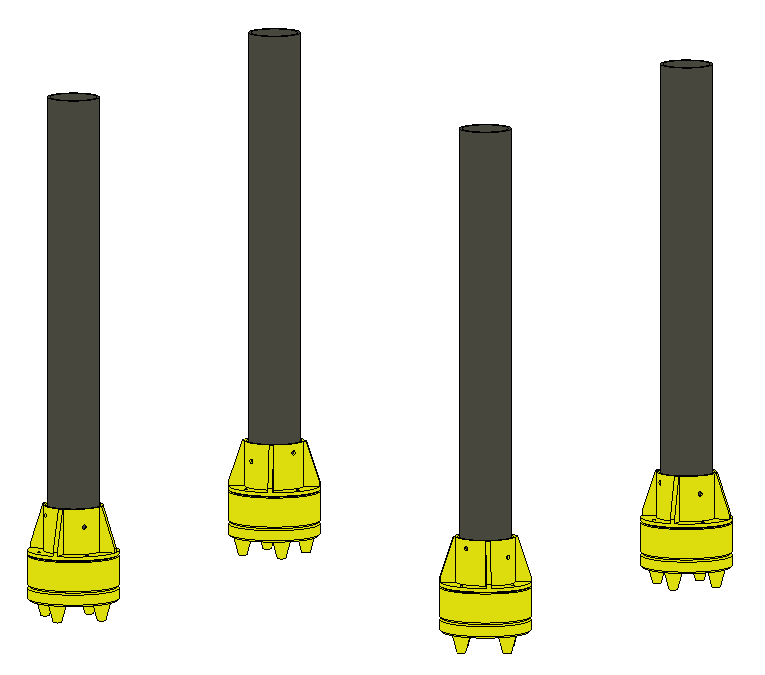
\includegraphics[width=0.4\textwidth]{images/requirements/no_text_ground_supports.png}
    \caption{Ground support elements for the GPR-20 robot.}
    \label{fig:considerations_ground_supports}
\end{figure}

\newpage
\section{Transport Recommendations}
Transport of the GPR-20 robot is required to fulfill its main objective: to acquire data in deactivated landmine fields. Transport should be done under certain conditions in order to prevent the robot from damaging. In the case of transporting towards a remote field, damage is very likely to spoil the data-acquisition activities. Otherwise, repairs for the robot would cost both time and resources. In general terms, actions should be taken to prevent damage of the robot. Table \ref{tab:transport_recommendations} presents recommendations for transporting the robot. Some of the recommendations are general while others are specific for each major component.

\begin{onehalfspacing}
    \begin{xltabular}{\textwidth}{|p{5cm}|X|}
        
        \hline \textbf{Part} & \textbf{Recommendation} \\ \hline
        \endhead
        
        \hline \textbf{Part} & \textbf{Recommendation} \\ \hline
        \endfirsthead
        
        \multicolumn{2}{|c|}{\textit{Continues on next page.}} \\ \hline
        \endfoot
        
        \caption{Transport recommendations for the GPR-20 robot.} \label{tab:transport_recommendations}
        \endlastfoot
        
        General & The used transport should provide an flat surface to place the components. If possible, the transport should provide the means to latch the parts using straps.  \\ \hline
        General & Transport should consider storage space for the personal computer, network switch, VNA and antennae. Storage should also be provided for the power supply if needed. \\ \hline
        Electronics Box & The electronics box should be transported laying over the its back side. The electronics box should not be transported over its bottom as it may damage the cables coming out of the electronics box. If straps can  be used, secure the electronics box from the PVC tube and the electronics box. Do not attach straps to touchscreen support. \\ \hline
        X-Axis & X-Axis should be transported with the universal mount located near the end of the support rods and the lead screw. The X-Axis will lay over the tip of the support rods and the SC12UU supports of the X-Axis auxiliary support. If straps are available, secure the X-Axis at two points of the support rods. \\ \hline
        Y-Axes & Transport of the Y-Axes is done with the axes laying down on their lateral sides. Left Y-Axis will lay down on the left side while right Y-Axis will lay down on the right side. Notice that transport side are the ones without the supports for the PVC tubes. This will prevent the axes from tipping over during transport. Right Y-Axis requires to secure the SC12UU bearings to prevent them from sliding over the support rods during transport. If straps are available, secure the Y-Axes at the support rods from both axes. \\ \hline
        Ground Support Elements & Ground support elements should be transported with their footer retracted. Lay the ground supports to prevent them from tipping over. If straps are available, secure them at the PVC tube where it inserts into the support element. \\ \hline
        VNA Holder & The VNA Holder lays over its front side i.e. the side in which the upper lid does not has openings. VNA and antennae should not be transported while mounted in the VNA holder. If straps are available, they should be attached to the support elements of the VNA holder. \\ \hline
        VNA & The VNA should be transported in its case. The VNA must not be in danger of falling or tipping over since it would damage the device. \\ \hline
    \end{xltabular}
\end{onehalfspacing}


\newpage
\section{Field Assembly}
This section presents the GPR-20 assembly guide. This section can be delivered as a standalone document in order to be used during each robot assembly. Please read the procedure before interacting with the robot and follow each step. Missing one step or doing it without the proper attention could lead to permanent damage of the robot.


\begin{onehalfspacing}
\begin{xltabular}{\textwidth}{|c|p{4cm}|X|}
    
    \hline  & \multicolumn{1}{c|}{\textbf{Name}} &\multicolumn{1}{c|}{\textbf{Description}} \\ \hline
    \endfirsthead
    
    \multicolumn{3}{|c|}{(continues on the next page)} \\ \hline
    \endfoot
    
    \endlastfoot
    
    $\square$ & Electronics Box Placement & Place the electronics box in front of you. The electronics box and the PVC tube should be located in theirs final location. \\ \hline
    $\square$ & Right Y-Axis Placement & Place the right Y-Axis perpendicular to the electronics box and its PVC tubing. The axis-end with the stepper motor should be near the right end of the electronics PVC tube. \\ \hline
    $\square$ & Left Y-Axis Placement & Place the left Y-Axis perpendicular to the electronics box and its PVC tubing. The axis-end with the stepper motor should be near the left end of the electronics PVC tube. \\ \hline
    $\square$ & Right Y-Axis Motor Connection & Connect the leading cables of the PVC tube to the connectors on the right Y-Axis. Check that cables of the same color are connected together: connecting cables of different colors can lead to permanent damage of the motor. \\ \hline
    $\square$ & Right Y-Axis and Electronics Mating & Identify the Y-Axis support from which cables come out. Insert the identified support into the electronics PVC tube. The support should be fully inserted into the tube without any cable being stuck. \\ \hline
    $\square$ & Left Y-Axis Motor Connections & Identify the motors cable sets from the electronics PVC tube and the left Y-Axis. Each set of motor cables is identified with tags on both the electronics box and the left Y-Axis. Connect each corresponding set of cables from the left Y-Axis to the cables on the PVC tubing. Check that cables from the same color and the same tag are connected together: connecting cables of different colors and/or sets can lead to permanent damage of the motor. \\ \hline
    $\square$ & Left Y-Axis Endstop Sensors Connections & Identify the endstop sensors cable sets from both the electronics PVC tube and the left Y-Axis. Connect each corresponding set of cables together. Make sure to connect cables from the same color and the same tag together: connecting cables of different colors and/or sets can lead to permanent damage of the sensors. \\ \hline
    $\square$ & Left Y-Axis VNA Connections & Identify the connections for the VNA power supply and the Ethernet data on both the left Y-Axis and the PVC tube.  Connect each corresponding set of cables together. \\ \hline
    $\square$ & Left Y-Axis and Electronics Mating & Insert the left Y-Axis support from which the cables come out. Insert the identified support into the electronics PVC tube. The support should be fully inserted into the tube without any cable being stuck. \\ \hline
    $\square$ & Standalone Arm mating & Insert the ends of the standalone PVC tube into the support elements of both the left and right Y-Axis arms. The supports must be fully inserted into the PVC tube. By this point, the edges of the Cartesian arm must be fully installed. \\ \hline
    $\square$ & X-Axis Arm Placement & Place the X-Axis arm parallel to the Electronics Box arm inside the robot. The X-Axis support can rest on the left Y-Axis arm rods and linear screw. The open end of the X-Axis arm can rest on the work surface. At this point you have to identify the bearings and the nut in the right Y-Axis arm. The nut must be somewhere close to the same distance of the right Y-Axis arm nut. There is no need to align the left Y-Axis bearings yet. \\ \hline
    $\square$ & X-Axis Open End Mating & Lift the X-Axis linear rods and linear screw. Insert the linear rods into the X-Axis motor mount linear rod supports. Mind the linear screw while inserting the rods. The three elements must be inserted at the same time. Once the elements are inserted, secure them by tightening the screws on the supports and coupling. The X-Axis support must lie over the left Y-Axis linear rods by this point.  \\ \hline
    $\square$ & X-Axis Support Mating & Place the X-Axis support over the nut in the right Y-Axis arm. If the nut is misaligned to the corresponding support holes, you can adjust the position by rotating the nut. Use two four-millimeter screws (M4) to secure the X-Axis support to the nut. Place the bearings below the support and align them to the corresponding holes. Secure the bearings to the X-Axis support with eight five-millimeter screws (M5). \\ \hline
    $\square$ & Ground Supports Placement & Place each group support component near the Y-Axis support elements. You will need to have the ground supports close to the robot in order to place them in their position. The recommended placement is having the ground support elements in the ground, perpendicular to the standalone and electronics arms and with the free-end pointing towards the robot. \\ \hline
    $\square$ & Standalone Arm Ground Supports Mating & Place yourself in the middle of the standalone arm and make sure that you can reach at least one ground support component. Lift the robot from the standalone arm and place a ground support in the Y-Axis support element that you find easier. Without letting go the robot arm, place the second ground support component in the remaining Y-Axis support element. The robot will be tilted and the ground support elements will be in tension until the second set is placed. \\ \hline
    $\square$ & Electronics Arm Ground Support Mating & Place yourself in front of the electronics box and make sure that you can reach at least one ground support component. Lift the robot from the electronics box and place a ground support in the Y-Axis support element that you find easier. Without letting go the electronics arm, place the second ground support element in the remaining Y-Axis support. \\ \hline
    $\square$ & Ground Support Components Check & Check that each ground support component is properly inserted in the Y-Axis support element. You must also check that the ground support components are perpendicular to the robot Cartesian arm. Adjust the ground support components screw to level the robot if necessary. By the end of the checks you must feel that the robot is stable and well supported. \\ \hline
    $\square$ & GPR Support Structure Preparation & Remove the antennae support from the GPR Support Structure by unscrewing the four five-millimeter (M5) screws. Pull the cables from the drag chain to allow the antennae support to rest in the floor while installing the GPR structure. Remove the auxiliary support by removing the four three millimeter (M3) screws. Insert the four five-millimeter (M5) screws in the universal mount holes.  \\ \hline
    $\square$ & GPR Support Structure Mount & Place the upper part of the GPR Support Structure in the X-Axis universal mount. Lift the GPR Support Structure and align the universal mount screws to the previously inserted screws. Tight one screw from one side into the universal mount. Without letting go the GPR Support Structure, tight another screw from the other side. At this point, the GPR structure should keep in place. Tight the remaining screws into the universal mount. \\ \hline
    $\square$ & GPR Support Structure Setup & Place the auxiliary support of the GPR Support Structure into position with the four previously removed three-millimeter (M3) screws. Check that the damper elements are secured in place. Install the antennae support with the previously removed five-millimeter (M5) screws. Check that the assembly is properly secured. \\ \hline
    $\square$ & X-Axis Drag Chain Setup & Put the GPR Support Structure cables into the universal mount drag chain end. Secure them by attaching the upper part of the end link. Pull the drag chain into the end link and plug it into position. Put the cables into the drag chain end in the X-Axis motor mount. Secure them with the upper part of the end link. Plug the corresponding end of the drag chain on the end link. \\ \hline
    $\square$ & VNA Setup & Remove the upper lid from the GPR support structure. Place the VNA minding the connections to the antennae. Place the VNA adapter next to the VNA and connect the power supply. Connect the microwave cables and the power supply to the VNA. Close the lid and secure it with the previously removed screws. \\ \hline
    $\square$ & Antennae Setup & Mount each antenna into the motors and secure them by tightening the screws on the antenna adapter. Connect the loose end of the microwave cables to the antennae.  \\ \hline
    $\square$ & Rest & The field setup assembly can be exhausting. Take a minute to rest and admire the robot you have assembled. By this point, the GPR-20 robot has been assembled. However some additional setup is required for the robot to operate. \\ \hline 
    $\square$ & Network switch & Place the network switch near the robot. Make sure that the network switch is safe from the environment. The network switch will have three connections: to the GPR-20 robot on-board computer, to the VNA, and to the personal computer. Two network cables come from the electronics box of the GPR-20 robot. Connect the Ethernet cables to the network switch.  \\ \hline
    $\square$ & Personal computer & Place the personal computer near the robot. Make sure that the personal computer is safe from the environment. The personal computer will connect to the network switch using an Ethernet cable. Connect the cable to the network switch. \\ \hline
    $\square$ & Power the setup & Connect the power cord of the personal computer, network switch, and GPR-20 robot to the power source. Allow for the three devices to initialize. The whole system is ready for testing to take place. \\ \hline
\end{xltabular}
\end{onehalfspacing}

\newpage
\section{Tools Configuration}
Two devices are used for the data-acquisition process: an on-board computer and a personal computer. The on-board computer is configured in such a way that it automatically starts all the required tools that are run on it. However, the personal computer is assumed not to execute this process. This section will focus on the tools initialization and check process. Although the personal computer does not launch the tools automatically on startup, the process of starting them requires few steps. The first step consists of sourcing the Robotic Operating System (ROS) workspace with the required tools. The workspace is sourced by executing: 
\begin{verbatim}
    $ source ~/gpr20_ws/devel/setup.bash
\end{verbatim}
Sourcing the workspace allows ROS to \textit{know} that there are packages i.e. tools available in the \texttt{gpr20\_ws} directory. The available packages on the workspace should be \textit{gpr20\_data\_acquisition}, \textit{gpr20\_data\_processing}, and \textit{gpr20\_msgs}. The next step is to configure ROS to connect with the on-board computer of the GPR-20 robot. This requires the user to know the GPR-20 on-board computer and personal computer IP addresses. Several third-party tools are available to scan the network and identify the IP addresses. To configure ROS to connect over multiple machines it is necessary to execute:
\begin{verbatim}
    $ export ROS_IP=<personal_computer_ip> 
    $ export ROS_MASTER_URI=http://<on-board_computer_ip>:11311 
\end{verbatim}
The final step is to launch the personal computer tools. These tools are launched via a script that eases the process. The script is located in the \textit{gpr20\_msgs} packages. To launch the script execute:
\begin{verbatim}
    $ roslaunch gpr20_msgs pc_utilities
\end{verbatim}
After launching the personal computer tools, checks should be performed to ensure the connectivity between computers and that all the tools are initialized. Table \ref{tab:tools} presents the checklist for the GPR-20 software. Once all the tools have been checked, the tools are ready for the data acquisition process to take place. The tools checklist should be completed after executing the \texttt{rosnode list} command.

\begin{xltabular}{\textwidth}{|c|X|}
    
    \hline & \textbf{Tool} \\ \hline
    \endhead
    
    \hline & \textbf{Tool} \\ \hline
    \endfirsthead
    
    \hline \multicolumn{2}{|c}{\textit{Continues in next page.}} \\ \hline
    \endfoot
    
    \caption{Tools checklist for GPR-20 software.} \label{tab:tools}
    \endlastfoot
    
    $\square$ & \textbf{Axis Driver:} there should be three (3) instances of the axis driver node. The instance of the X axis should have the name \textit{gpr20\_x\_axis}. The instance of the Y axis should have the name \textit{gpr20\_y\_axis}. Finally, the instance of the Z axis should have the name \textit{gpr20\_z\_axis}. \\ \hline
    $\square$ & \textbf{Height Sensor Driver:} there should be a single instance of the height sensor driver node. \\ \hline
    $\square$ & \textbf{VNA Acquisition:} there should be a single instance of the VNA acquisition node. \\ \hline
    $\square$ & \textbf{VNA Processing:} there should be a single instance of the VNA Processing node \\ \hline
    $\square$ & \textbf{Main Control:} there should be a single instance of the main control. \\ \hline
    $\square$ & \textbf{User Interface:} there should be a single instance of the user interface. \\ \hline
\end{xltabular}


\newpage
\section{Field Testing}
The field testing aims to check that the robot is capable of acquiring data. Three (3) procedures are intended to be executed by the robot user to check the robot capabilities prior to the data acquisition. The first procedure is checking the robot pose, which checks that the robot is leveled against the surface. The second procedure is calibrating the VNA instrument which is used to acquire the data. The third and final procedure is acquiring data under a known condition to check the robot operation. Fill the following table for robot keeping purpose prior to every surveying.

\begin{onehalfspacing}
    \begin{xltabular}{\linewidth}{|l|X|}

        \endhead
    
        \endfirsthead
        
        \endfoot
        
        \endlastfoot
        
        \hline \textbf{Date:} & \\ \hline
        \textbf{Location:} & \\ \hline
        \textbf{Responsible:} & \\ \hline
    \end{xltabular}
\end{onehalfspacing}

\subsection{Checking the Robot Pose}
This test will check that the robot is leveled against the surface. In order to execute this test, a smart device is required. The smart device needs to have a leveling measurement application installed and calibrated. Check that the device measurements are consistent by testing it against a known leveled surface such as a table or a wall.

\begin{onehalfspacing}
\begin{xltabular}{\linewidth}{|c|p{4cm}|X|}

    \hline & \textbf{Name} & \textbf{Description} \\ \hline
    \endhead

    \hline & \textbf{Name} & \textbf{Description} \\ \hline
    \endfirsthead
    
    \multicolumn{3}{|c|}{\textbf{Continues on next page.}} \\ \hline
    \endfoot
    
    \caption{Robot pose check.} \label{tab:robot_pose}
    \endlastfoot
    
    $\square$ & Reset footers & Rotate the ground support elements footers until there is no gap between the footer and the support. \\ \hline
    $\square$ & Initial measurement & Place the smart device on top of the VNA cover. Make sure that the back of the smart device is completely against the cover. Open the level application. Check the angle in which the device lies. Angle: \_\_\_\_\_ $^{\circ}$. \\ \hline
    $\square$ & Robot leveling & If the angle is different from $0^{\circ}$, rotate the ground support elements footers until the angle is zero. \\ \hline
\end{xltabular}
\end{onehalfspacing}

\subsection{Calibrating the VNA Instrument}
Calibrate the VNA device according to the manufacturer manual and the available calibration kit. The GPR-20 is designed for the Anritsu MS2026C VNA. The calibration of the device is done using a calibration kit. Reference of the calibration kit is TOSLN50A-18. The recommended calibration for the VNA is to to acquire $512$ frequency data points within $600$MHz and $6.0$GHz. Table \ref{tab:vna_calibration} presents the calibration process for the MS2026C VNA using the TOSLN50A-18 calibration kit. If using a different device and/or calibration kit, follow the manufacturer procedures to ensure that the calibration is done correctly and the device is ready to acquire data.

\begin{xltabular}{\textwidth}{|c|X|}

    \endhead
    
    \endfirsthead
    
    \endfoot

    \caption{Anritsu MS2026C calibration process using the TOSLN50A-18 calibration kit.} \ref{tab:vna_calibration}    
    \endlastfoot
    
    $\square$ & Turn on the VNA device and wait fifteen (15) minutes until it heats up. This is done to ensure that the device calibration will occur at its operating temperature. \\ \hline

\end{xltabular}

\subsection{Data Acquisition Test}
This test will check the data against a known survey condition. The condition consists of placing a metal sheet over the survey area and check the VNA response. A-Scans will be used to validate the data acquisition process. You will need a $50\times 50$ centimeters metal sheet for this test and the tester script.

\begin{onehalfspacing}
    \begin{xltabular}{\linewidth}{|c|p{4cm}|X|}
    
        \hline & \textbf{Name} & \textbf{Description} \\ \hline
        \endhead
    
        \hline & \textbf{Name} & \textbf{Description} \\ \hline
        \endfirsthead
        
        \multicolumn{3}{|c|}{\textbf{Continues on next page.}} \\ \hline
        \endfoot
        
        \caption{Data acquisition test.} \label{tab:data_acquisition}
        \endlastfoot
        
        $\square$ & Metal sheet placement & Place the metal sheet in the middle of the survey area of the robot. Make sure that the metal place is well positioned against the ground. \\ \hline
        $\square$ & Power the robot & Connect the robot to the power source. Allow the user interface to load in the touchscreen. Make sure that the robot is connected to the network switch.  \\ \hline
        $\square$ & Power the personal computer & Turn on the personal computer and connect it to the network switch. \\ \hline
        $\square$ & VNA network connection & Connect the Vector Network Analyzer network cable to the network switch. \\ \hline
        $\square$ & Launch personal computer utilities & Start the personal computer utilities (\texttt{\$ roslaunch gpr20\_msgs pc\_utilties}). The command line should display an \texttt{OK} message. \\ \hline
        $\square$ & Start test data acquisition & Navigate to the tests tab in the user interface. Click on the data acquisition test. The robot will move to the center of the survey area and will acquire data in $100$ different coordinates. Once data is acquired, the robot will return to the homing position. \\ \hline
        $\square$ & Check results & Data will be stored in the GPR-20 data directory (\texttt{/home/<user>/GPR20/data/}) of the personal computer. Survey will be in a folder with the date and time at the start of the survey (\texttt{\%DD\_\%MM\_\%YYYY\_\%HH\_\%MM}). Check that one hundred (100) data files are in the folder before proceeding.  \\ \hline
        $\square$ & Execute test script & Execute the test script with the data folder as parameter (\texttt{python data\_acquisition\_test --path=<path\_to\_data>}). If test fails, calibrate the VNA device. \\ \hline
    \end{xltabular}
\end{onehalfspacing}

\newpage
\section{Parameters and Acquisition}
The surveying process depends on the defined parameters from the user. Two (2) major groups of parameters are defined for the survey: VNA parameters and survey parameters. VNA parameters refer to the device configuration regarding the data acquisition. Survey parameters refer to the values used for defining the grid points in the sampling process. Both parameters have huge implications on the data acquisition process and the data itself. This section will present a brief discussion on the considerations regarding the parameters. Table \ref{tab:parameters_considerations} presents the discussion on the parameters.

\begin{xltabular}{\textwidth}{|l|X|}
    
    \hline \textbf{Parameter} & \textbf{Considerations} \\ \hline
    \endhead
    
    \hline \textbf{Parameter} & \textbf{Considerations} \\ \hline
    \endfirsthead
    
    \multicolumn{2}{|c|}{\textit{Continues on next page.}} \\ \hline
    \endfoot
    
    \caption{GPR-20 survey parameters considerations.} \label{tab:parameters_considerations}
    \endlastfoot
    
    Start Frequency & Defines the minimum frequency that will be used in the VNA for acquiring the data. The effective frequency value i.e. the real frequency in which data will be sampled depends on the VNA calibration. The device will use the closest frequency value that is available after the VNA calibration. \\ \hline
    Stop Frequency & Defines the maximum frequency that will be used in the VNA for acquiring the data. Similar to the start frequency, the effective frequency depends on the VNA calibration. The device will use the closes available frequency value defined on calibration. \\ \hline
    Frequency Points & Defines the frequency points that will be used in the data acquisition process. The VNA will use the frequency points defined in the calibration process. It might be possible for the device to use a different amount of frequency points than the ones defined by the user. \\ \hline
    X/Y Start Coordinate & Defines the initial coordinate for either the X or Y axes. The coordinates are referenced from the left Y axis driver component with positive values oriented along the axes. The origin for the coordinates is referenced with the endstop sensors. It must be noted that each axis has its own start coordinate field. \\ \hline
    X/Y Stop Coordinate & Defines the final coordinate for either the X and Y axes. The coordinates are referenced from the left Y axis driver component. Positive axis values are oriented towards the axes. In other words, the endstop sensors provide the zero coordinate. It must be noted that each axis has its own start coordinate field. \\ \hline
    X/Y Points & Defines the physical points that the axes will visit. The minimum amount of points that an axis can visit is two (2). There is no predefined maximum amount of points that an axis can visit. Two considerations are presents for these fields. The first one being that each axis has its own field for the physical points. The second one is that the delta distance i.e. the distance between points is calculated with the difference between the start and stop coordinates divided by the number of points minus one: $(X_{end} - X_{start})/(N_{points} - 1)$.  \\ \hline
\end{xltabular}

Each parameter is defined in the user interface of the robot. The user interface is displayed in the GPR-20 touchscreen. The user can define a step value for the input operation. Available steps are $0.1$, $1$, $10$ and $100$. This is done in order to reduce the required interactions of the user to input the parameters. Frequency parameters fields are defined in Gigahertz (GHz, $1\times 10^{9}$Hz). Coordinate fields are defined in millimeters. In order to start a survey, the user is required to input the parameters in the user interface and send the start command. The robot will execute the homing procedure and then will start moving and acquiring the data. Once the data acquisition process finishes, the robot will return to the home position. The user is required to supervise the data acquisition process. 


\newpage
\section{Survey Supervision}
Supervision of the data acquisition process is critical to ensure that the process is being executed as intended. There are two possible failures that can occur during the survey process: software and hardware. GPR-20 software has been thoroughly debugged in order to prevent failures during the sampling process. However, hardware failures can occur during the sampling process. Being able to identify failures as soon as possible is a strategy that aims to save time. Table \ref{tab:supervision} presents the checklist that the user has to execute every hour during the sampling process.

\begin{xltabular}{\textwidth}{|c|X|}

    \hline & \textbf{Check} \\ \hline
    \endhead
    
    \hline & \textbf{Check} \\ \hline
    \endfirsthead
    
    \multicolumn{2}{|c|}{\textit{Continues on next page.}} \\ \hline
    \endfoot
    
    \caption{GPR-20 survey supervision checklist.} \label{tab:supervision}
    \endlastfoot
    
    $\square$ & \textbf{Check X-Axis movement:} check that the X axis is moving. The axis and the motors should spin smoothly. The axis could not move if dirt is present in the lead screw and/or the support rods. Make sure that the axis position is consistent with the current coordinate. \\ \hline
    $\square$ & \textbf{Check Y-Axis movement:} check that both supports of the Y-Axis are moving. Both supports and their motors should be moving smoothly. Check that both supports are in the same coordinates and with the X-Axis perpendicular to both of them. Check for dirt in the lead screw and the support rods. \\ \hline
    $\square$ & \textbf{User Interface:} check that the user interface is responsive. Change tabs and check that feedback data is being updated continuously. \\ \hline
    $\square$ & \textbf{Data Storage:} check the data in the personal computer. Ensure that data is being stored and files contain values in the CSV format. \\ \hline
    
\end{xltabular}


\newpage
\section{Field Disassembly}
This section presents the field disassembly guide for the GPR-20 robot. Please read the whole procedure before executing it. This section can be used as a standalone document in order to provide the field checklist. Keep in mind that failing to execute this procedure could result in permanent damage to the robot.

\begin{onehalfspacing}
    
\begin{xltabular}{\textwidth}{|c|p{4cm}|X|}

    \hline & \textbf{Name} & \textbf{Description} \\ \hline
    \endhead
    
    \hline & \textbf{Name} & \textbf{Description} \\ \hline
    \endfirsthead
    
    \multicolumn{3}{|c|}{\textit{Continues in next page.}} \\ \hline
    \endfoot
    
    \endlastfoot
    
    \hline
    $\square$ & Power down the devices & Power down the personal computer and the network switch. Wait for the devices until they shut down. Unplug the GPR-20 robot, VNA device, personal computer and network switch. \\ \hline
    $\square$ & Personal computer storage & Unplug the personal computer from the power source and the network switch. The personal computer now can be stored. \\ \hline
    $\square$ & Network switch storage & Unplug the network switch from the power source. Unplug the network cables from the switch. The switch now can be stored. \\ \hline
    $\square$ & Antennae removal & Disconnect the microwave cable from the antennae connector. Unscrew the two (2) M3 tightening screws in each antennae adapter. Remove the antennae with the adapter from the motor shafts at the bottom of the VNA holder. You can now store the antennae. \\ \hline
    $\square$ & VNA removal & Disconnect the Ethernet, power and microwave cables from the VNA. You can now store the microwave cables. Unscrew the four (4) M5 screws at the bottom of the upper lid in the VNA holder. Lift the VNA holder upper lid and set aside. Remove the VNA from the holder. You can now store the VNA. Do not attach the VNA upper lid back to the VNA holder. \\ \hline
    $\square$ & X-Axis drag chain unplug & Disconnect the two (2) motor connectors, VNA power and VNA Ethernet cable at the VNA holder and the X-Axis support.  \\ \hline
    $\square$ & X-Axis drag chain removal & Unlatch the X-Axis drag chain from the end links at the VNA holder and the X-Axis driver support. Remove the drag chain and store it. \\ \hline
    $\square$ & VNA Holder removal & Unscrew the four (4) M5 screws at the top of the VNA mounting plate. This will detach the mounting plate from the VNA holder supports. Unscrew the four (4) M5 mounting screws from the sides of the VNA holder supports. The lower part of the VNA holder will detach from the universal mount. Remove the lower part of the VNA holder. Attach the VNA mounting plate back to the VNA holder supports via the previously removed four (4) M5 screws. Attach the upper lid back to the VNA mounting plate with the remaining four (4) M5 screws. You can now store the VNA holder major group. \\ \hline
    $\square$ & X-Axis auxiliary support detaching & Remove the eight (8) M5 screws from the X-Axis auxiliary support element. Remove the four (4) remaining M4 screws. Be careful with the nuts from the M4 screws. Store the screws and nuts for future use. \\ \hline
    $\square$ & X-Axis removal & Unscrew the tightening screws at the linear rod supports and lead screw bearing from the X-Axis driver element. These will loose the linear rods and lead screw. Carefully lift the X-Axis major group while separating the linear rods and lead screw from their supports. The X-Axis major group is now ready for storage. \\ \hline
    $\square$ & Y-Axis drag chain disconnection & Disconnect the three (3) motor connectors, endstop sensor connector, VNA Ethernet cable and power cord from both the X-Axis driver element and the left Y-Axis driver.  \\ \hline
    $\square$ & Y-Axis drag chain removal & Unlatch the Y-Axis drag chain from the end links at the X-Axis driver and Y-Axis left driver. Store the Y-Axis drag chain. \\ \hline
    $\square$ & Ground support removal & Lift the driver side from the GPR-20 robot i.e. the side with the electronics box and remove the two (2) ground support elements. Carefully lower that side until it settles into the ground. Lift the other side of the robot and remove the ground support elements. Settle the robot into the ground. You can now store the ground support elements. \\ \hline
    $\square$ & Auxiliary PVC tube removal & Move the left and right Y-Axis auxiliary supports in order to free the auxiliary PVC tube. Remove and store the PVC tube. \\ \hline
    $\square$ & Electronics box separation & Move the left and right Y-Axis driver elements. The PVC tube from the electronics box should detach from the Y-Axis drivers. Be careful with the cables that run along the electronics box PVC tube. Leave the electronics box detached. \\ \hline
    $\square$ & Electronics box disconnection & Disconnect the four (4) motor connectors, two (2) endstop sensors connectors, VNA power and Ethernet cables from the left Y-Axis driver. Disconnect the motor connector at the right Y-Axis driver. You can now remove and store the electronics box. The Y-Axes will also be ready for storage. \\ \hline
\end{xltabular}
\end{onehalfspacing}

\end{document}
